\documentclass[addpoints,11pt]{exam}

\usepackage{alltt}
\usepackage[margin=1in]{geometry}   % set up margins
\usepackage[T1]{fontenc}
\usepackage[usenames,dvipsnames]{xcolor}
\usepackage{enumerate}              % fancy enumerate
\usepackage{amsmath}                % used for \eqref{} in this document
\usepackage{amsthm}
\theoremstyle{definition}
\newtheorem{exmp}{Example}[section]
\usepackage{verbatim}               % useful for \begin{comment} and \end{comment}
\usepackage{eurosym}                % used for euro symbol
\usepackage{caption} 
\usepackage{graphicx}
\graphicspath{{Figures/}}
\usepackage{subcaption}
\usepackage{color}
\usepackage{float}
\usepackage{amssymb}
\usepackage{sgamevar}
\usepackage{sgame}
\usepackage[colorlinks=true]{hyperref}
\hypersetup{colorlinks=true, citecolor=ForestGreen, linkcolor=BlueViolet, urlcolor=Magenta}

%Solutions or nah (blank next two lines out for no solutions, unblank #3)
%\printanswers
%\newcommand{\dd}[1]{\par {\textbf{\textcolor{red}{#1}}}}
\newcommand{\dd}[1]{}  


\setlength\parindent{0pt}
\unframedsolutions
\SolutionEmphasis{\color{red}}
\CorrectChoiceEmphasis{\color{red}}
\renewcommand{\choicelabel}{(\alph{choice})}
\newcommand{\blank}[0]{\underline{\hspace{3cm}}}
\pointformat{\bfseries[\thepoints]}
\pointpoints{pt}{pts}
\pointsinrightmargin


\begin{document}


\title{\textbf{Exam 1} \dd{Solutions} \\ \vspace{2 mm} {\large ECON 101-002}}
\author{Summer 2017}
\date{}
\maketitle

\makebox[\textwidth]{Name:\enspace\hrulefill}
\\

\makebox[\textwidth]{ONYEN:\enspace\hrulefill}
\\

\makebox[\textwidth]{PID:\enspace\hrulefill}
\\

\makebox[\textwidth]{Honor Code Signature:\enspace\hrulefill}


\section*{Multiple Choice [2.5 pts each]}

Choose the option that best answers the question given.

\begin{questions}
	
		
\question Table \ref{MC17} shows the quantity supplied and demanded at certain prices.


\begin{table}[h!]
	\caption{Prices and Quantities}
	\centering
	\begin{tabular}{  c | c | c} 
		
		Price & $Q_d$ & $Q_s$ \\
		\hline
		\$10 & 50 & 30 \\
		\$12 & 45 & 35 \\
		\$14 & 40 & 40 \\
		\$16 & 35 & 45 \\
		\$18 & 30 & 50 \\
	\end{tabular}
	\label{MC17}
\end{table}

If there is currently a surplus of 15 units, then the price in the market must be

\begin{choices}
	\choice less than \$14.
	\choice greater than \$14, but less than \$16.
	\CorrectChoice greater than \$16, but less than \$18.
	\choice greater than \$18.
\end{choices}

\newpage		
	

\question Refer to Figure \ref{MC2}.


\begin{figure}[H]
	\centering
	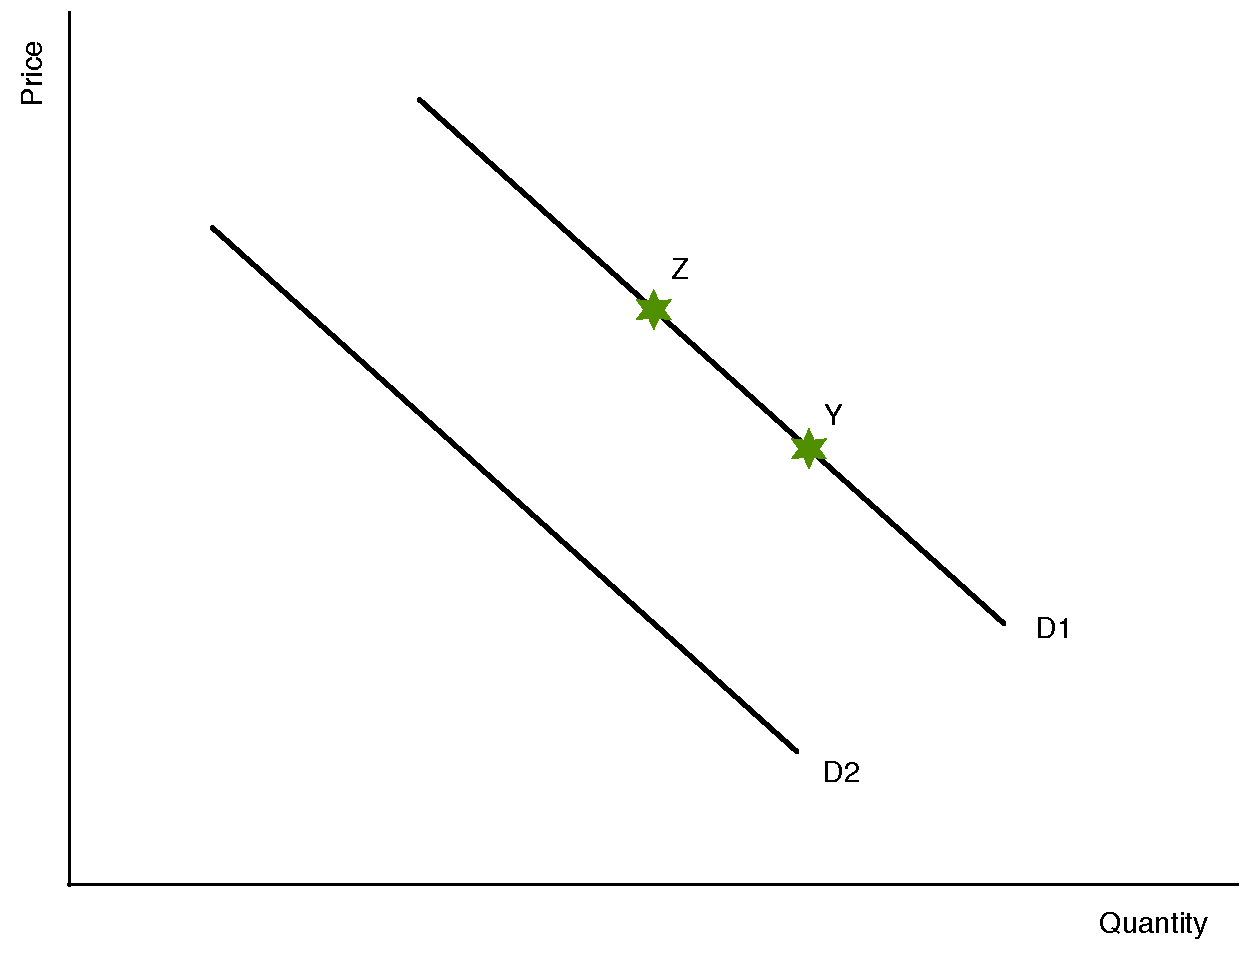
\includegraphics[scale=.40]{Exam1_MC2.pdf}
	\caption{Demand for Shrimp}
	\label{MC2}
\end{figure}

	All else equal, an increase in the income of buyers who consider shrimp to be an inferior good would cause a move from
		
		\begin{choices}
			\CorrectChoice D1 to D2.
			\choice Y to Z.
			\choice Z to Y.
			\choice D2 to D1.
		\end{choices}
		

	\question A non-congested toll road is a \blank because it is \blank.
	
	\begin{choices}
			\choice common resource; excludable and rival
			\choice private good; excludable and rival
			\choice public good; non-excludable and non-rival
			\CorrectChoice club good; excludable and non-rival
	\end{choices}


	\question Since chocolate chip cookies and oatmeal raisin cookies are substitutes, the cross-price elasticity of demand between the goods is 
	
	\begin{choices}
		\choice negative.
		\choice zero.
		\CorrectChoice positive.
		\choice impossible to discern without more information.
	\end{choices}


\newpage

\question Chocolate chip cookies and milk are complements. If the supply of chocolate chip cookies decreases, then the equilibrium price of milk will \blank and the equilibrium quantity will \blank.

\begin{choices}
	\choice increase; decrease
	\CorrectChoice decrease; decrease
	\choice decrease; increase
	\choice increase; increase
\end{choices}
	
	
\question The government of Tarheelia is debating over how to fund national defense, a public good. There are 40 individuals in the country, and each person places a value of \$0.30 on each dollar spent on national defense.

Under policy 1, the government asks individuals to voluntarily contribute towards the national defense fund. Under policy 2, a \$15 tax would be imposed on each individual. Individuals would each contribute \blank towards national defense under policy 1, while under policy 2 individuals would be \blank better/worse off relative to policy 1.

\begin{choices}
\choice \$0; \$180
\CorrectChoice \$0; \$165
\choice \$0.30; $-$\$15
\choice \$0; $-$\$15
\choice \$0.30; \$165
\end{choices}

\question The United States currently produces guns and butter. Table \ref{MC22} shows possible combinations of the two goods the US can produce in a given week (in thousands). 

\begin{table}[h!]
	\caption{Weekly Production of Guns and Butter}
	\centering
	\begin{tabular}{  c| c} 
		
		Guns & Butter \\
		\hline
		8 & 50 \\
		$x$ & 40  \\
		18 & 30 \\
	\end{tabular}
	\label{MC22}
\end{table}

If resources in the US are specialized such that some are better suited to producing guns and others are better suited for butter production, then a possible value for $x$ might be

\begin{choices}
	\choice 10
	\choice 12
	\choice 13
	\CorrectChoice 16
\end{choices}
	

		
\uplevel{Refer to Figure \ref{MC16}, which shows the market for laptop computers, for questions \ref{q5} - \ref{q6}.}

\begin{figure}[H]
	\centering
	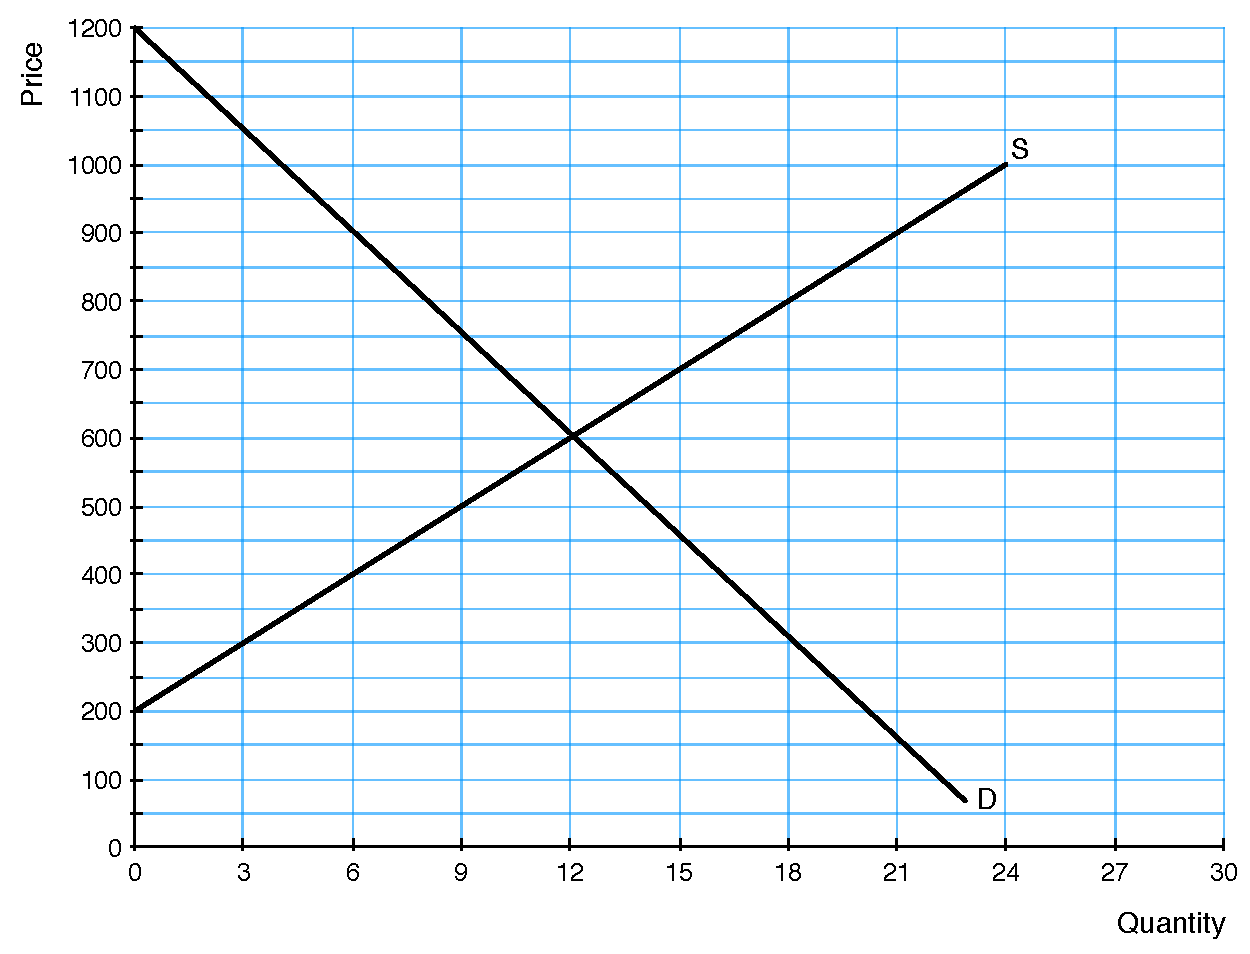
\includegraphics[scale=.40]{Exam1_MC16.pdf}
	\caption{Market for Laptops}
	\label{MC16}
\end{figure}

\question \label{q5} Suppose the government imposes a tax on this market such that the quantity bought and sold after the tax is imposed is 9 laptops. Thus, the size of the per-unit tax is \blank and the burden of the tax falls more heavily on \blank.

	\begin{choices}
		\choice \$250; sellers
		\choice \$750; buyers
		\choice \$750; sellers
		\CorrectChoice \$250; buyers
	\end{choices}

\question As a result of this tax, consumer surplus in this market will 

\begin{choices}
	\choice decrease by \$4,050
	\choice decrease by \$3,150
	\CorrectChoice decrease by \$1,575
	\choice decrease by \$2,025.
\end{choices}
	
\question \label{q6} The government decides to repeal the tax and instead provides a per-unit subsidy of \$500 to consumers. As a result of the subsidy, the deadweight loss in the market will be

\begin{choices}
	\CorrectChoice \$1,500.
	\choice \$2,000.
	\choice \$3,000.
	\choice \$2,500.
	\choice \$0.
\end{choices}
	

\newpage	
	
	\question Consider Figure \ref{MC19}. 
	
	\begin{figure}[H]
		\centering
		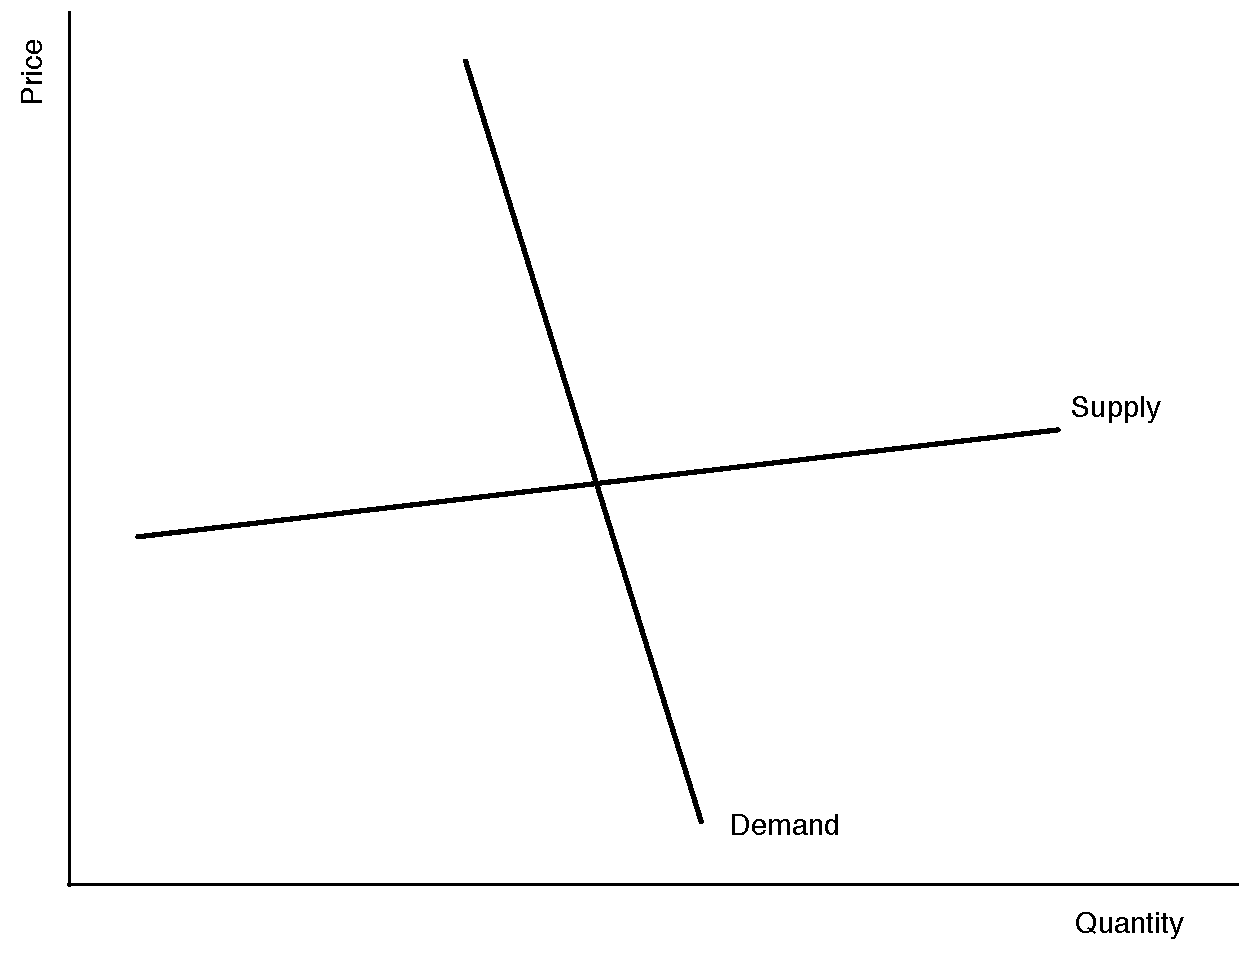
\includegraphics[scale=.40]{Exam1_MC19.pdf}
		\caption{Market for Coke}
		\label{MC19}
	\end{figure}
	
	If the government provides a \$15 per unit subsidy on sellers in this market, 
	
	\begin{choices}
		\choice the benefit of the subsidy will be split evenly between buyers and sellers in the market.
		\choice the benefit of the subsidy will be greater for sellers than for buyers in the market.
		\CorrectChoice the benefit of the subsidy will be greater for buyers than for sellers in the market.
	\choice the split of the subsidy benefit cannot be determined from this information. 
	\end{choices}

	
	\question Table \ref{SA2} shows the willingness to pay and costs of five sellers and buyers in the market for new textbooks. Each buyer would like one textbook and each seller has one book to sell.

\begin{table}[ht]
	\caption{WTP and Seller Costs for Textbooks}
	\centering
	\begin{tabular}{  c| c} 
		
		WTP   & Seller Costs \\
		\hline
		\$180 & \$85 \\
		\$150 & \$150 \\
		\$100 & \$100 \\
		\$200 & \$125 \\
		\$125 & \$60 \\
	\end{tabular}
	\label{SA2}
\end{table}

If a price floor of \$180 is imposed in this market, the deadweight loss incurred as a result of this price control is 

\begin{choices}
	\choice \$0.
	\choice \$95.
	\CorrectChoice \$50.
	\choice \$235.
	\choice \$180.
\end{choices}

\newpage
		
	
	\question Figure \ref{MC23} shows the demand curve for Fanta.
	
	\begin{figure}[H]
		\centering
		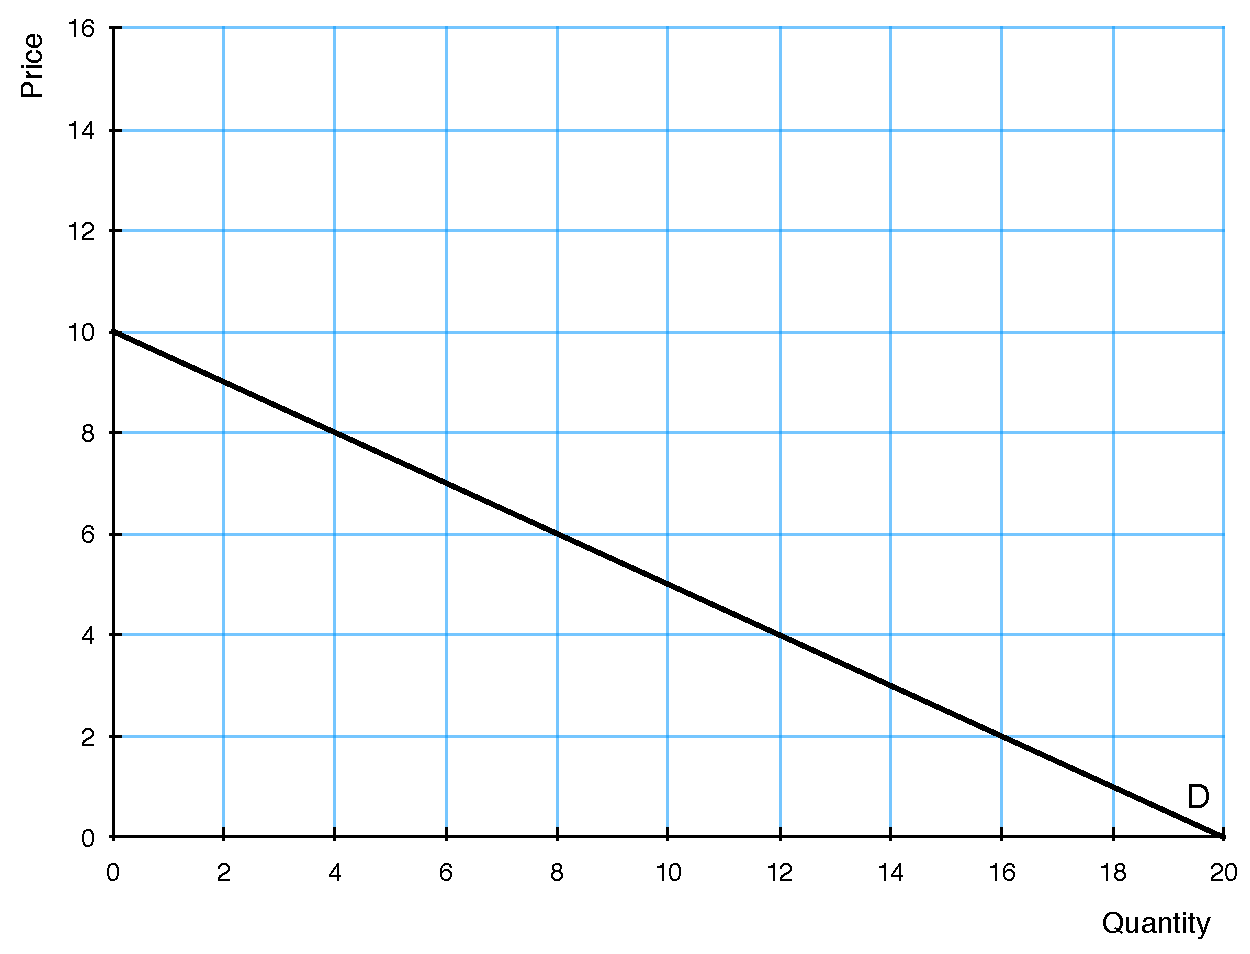
\includegraphics[scale=.40]{Exam1_MC22.pdf}
		\caption{Demand for Fanta}
		\label{MC23}
	\end{figure}
	
	If the price of Fanta increases from \$2 to \$4, consumer surplus will
	
	\begin{choices}
			\choice increase by \$28.
			\CorrectChoice decrease by \$28.
			\choice decrease by \$36.
			\choice increase by \$36.
	\end{choices}
	
\uplevel{Use the following information to answer questions \ref{q8} - \ref{q9}. Suppose we are studying a market where each unit bought and sold incurs an external cost of \$3 on society. However, the sale of this good also provides an external benefit of \$5 per unit.}


\question \label{q8} In the absence of government intervention, the market will provide an amount

\begin{choices}
	\CorrectChoice smaller than the efficient output level.
	\choice greater than the efficient output level.
	\choice equal to the efficient output level.
	\choice Not enough information given.
\end{choices}


\question \label{q9} In order to induce the market to produce the efficient quantity, the government could 

\begin{choices}
	\choice impose a \$2 per-unit tax on sellers.
	\choice provide a \$5 per-unit subsidy to buyers. 
	\choice impose a \$3 per-unit tax on buyers.
	\CorrectChoice provide a \$2 per-unit subisdy to buyers.
	\choice None of the above.
\end{choices}

\newpage
		
\question Consider Figure \ref{MC25}. 

\begin{figure}[H]
	\centering
	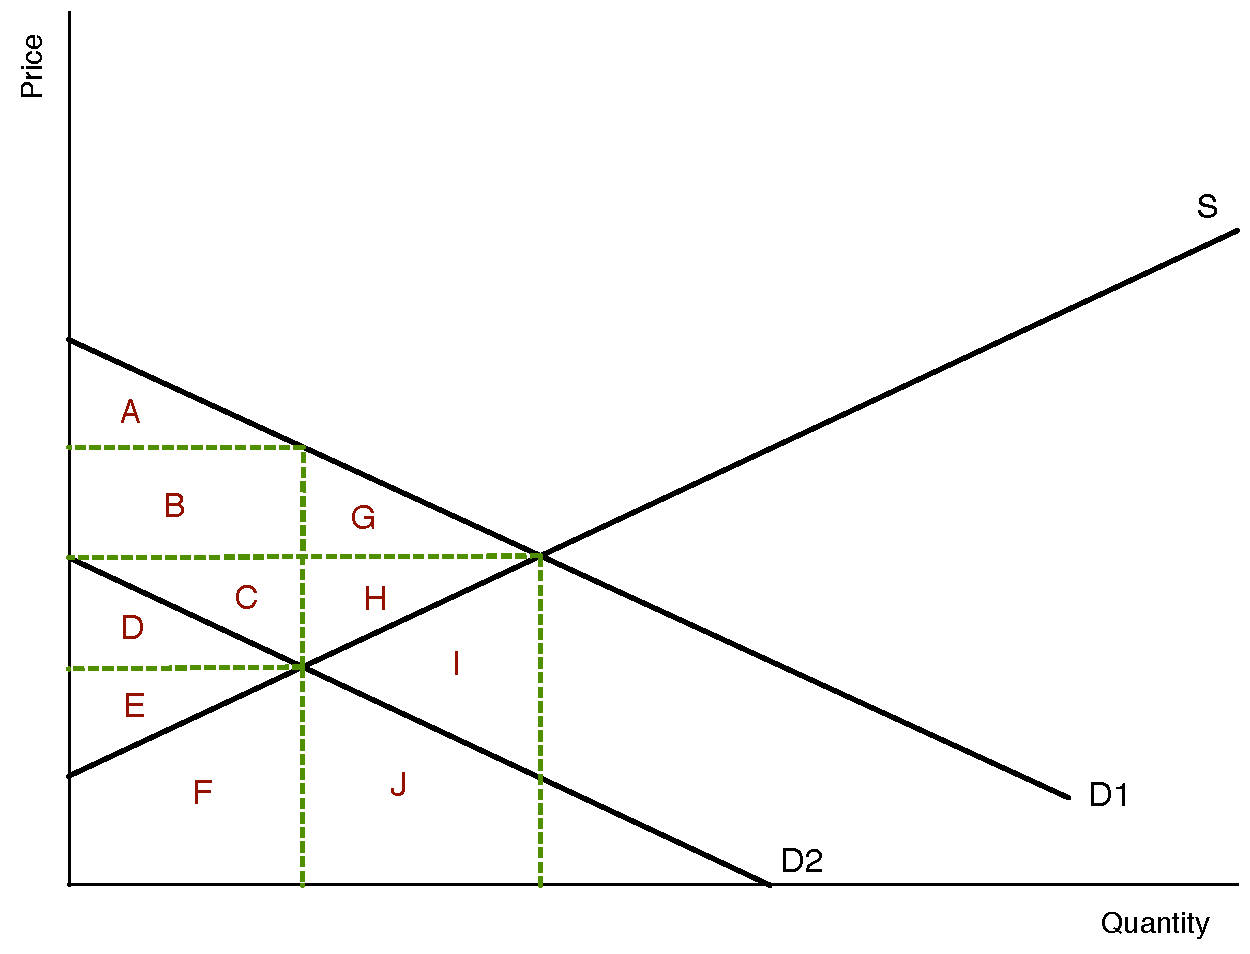
\includegraphics[scale=.40]{Exam1_MC25.pdf}
	\caption{Market for Fanta}
	\label{MC25}
\end{figure}



Suppose that the curve labeled D1 represents the social value curve in this market. In the absence of government intervention, total surplus in the market for Fanta is represented by the area

\begin{choices}
	\CorrectChoice A + B + C + D + E
	\choice A + B + C + D + E + G + H
	\choice A + B + C + G + H + I
	\choice D + E
	\choice None of the above.
\end{choices}









\question The market for Twist is currently at equilibrium and the price of the drink is \$1.00 per can. Under pressure from consumers, the government imposes a price ceiling of \$1.25 per can, leading to \blank in producer surplus and \blank in total surplus.

\begin{choices}
	\choice no change; an increase
	\CorrectChoice no change; no change
	\choice an increase; an increase
	\choice a decrease; a decrease
	\choice a decrease; no change
\end{choices}


\question If people purchase fewer beets when their incomes increase, then beets are a(n) \blank good and its income elasticity of demand is \blank.

\begin{choices}
	\choice normal; positive
	\choice inferior; positive
	\CorrectChoice inferior; negative
	\choice normal; negative
\end{choices}


\uplevel{Use Table \ref{MC8}, which shows the number of apples and pears Katie and Megan can produce in a day, and the information below to answer questions \ref{q12} - \ref{q14}.} 

\begin{table}[H]
	\caption{Number of units harvested per day:}
	\centering
	\begin{tabular}{ c|c|c} 
		
		& Apple & Pear \\
		\hline
		Katie & 6 & 18 \\
		Megan & 4 & 14 \\
	\end{tabular}
	\label{MC8}
\end{table}



The parties decide to trade and the following terms are proposed:

\begin{enumerate}[i.]
	\item 100 apples per 400 pears
	\item 200 pears per 100 apples 
	\item 65 pears per 22 apples
	\item 425 pears per 85 apples
\end{enumerate}


\question \label{q12} Given this information, it follows that 

\begin{choices}
	\choice Katie has the comparative advantage in producing both goods.
	\CorrectChoice Katie has the comparative advantage in producing apples, while Megan has the comparative advantage in pears.
	\choice Katie has the comparative advantage in producing pears, while Megan has the comparative advantage in apples.
	\choice Megan has the comparative advantage in producing both goods.
\end{choices}

\question \label{q13} Of the terms of trade proposed, how many would make Megan better off, but would make Katie worse off than without trade?

\begin{choices}
	\CorrectChoice 2
	\choice 1
	\choice 3
	\choice 0
	\choice 4
\end{choices}


\question \label{q14} Of the terms of trades proposed, how many would make both parties better off than without trade?

\begin{choices}
	\choice 3
	\choice 2
	\choice 4
	\CorrectChoice 0
	\choice 1
\end{choices}


\newpage

\question A per-unit tax of \$6 is imposed by the government. Use Table \ref{MC27} to answer the question below.

\begin{table}[h!]
	\caption{Unit Taxes}
	\centering
	\begin{tabular}{ c|c|c} 
		
		& Price with no tax & Price with \$6/unit tax on sellers \\
		\hline
		Price paid by buyers & \$55 & ? \\
		Price paid by sellers & \$55 & \$53.50  \\
	\end{tabular}
	\label{MC27}
\end{table}

Because of this tax, buyers are paying \blank per unit and sellers are receiving \blank per unit.

\begin{choices}
	\CorrectChoice \$4.50 more; \$1.50 less
	\choice \$1.50 more; \$4.50 less
	\choice \$3 less; \$3 more
	\choice \$2 more; \$4 less
\end{choices}


\uplevel{Refer to Table \ref{wtp}, which gives the costs to sell 1 lb of cauliflower for four individuals, for questions \ref{qblerg} - \ref{qblerg2}.}

\begin{table}[H]
	\caption{Costs for 1 lb Cauliflower}
	\label{wtp}
	\centering
	\begin{tabular}{  c|c    }    
		
		Seller   & Cost \\
		\hline
		Jasmine & \$4.00 \\
		Tyler & \$2.50 \\
		Deepak & \$3.00 \\
		Sarah & \$.50 \\
	\end{tabular}
	
\end{table} 

\question \label{qblerg} Suppose the price of cauliflower increases from \$2.00 to \$2.25. The \underline{increase} in producer surplus in the market as a result of this price change is 

\begin{choices}
	\choice \$0
	\choice \$0.75
	\choice \$0.50
	\CorrectChoice \$0.25
\end{choices}

\question \label{qblerg2} There are four buyers in the market for cauliflower. Demand is perfectly elastic and each buyer is willing to pay \$3.00 for one pound of cauliflower. Total surplus in the market is thus

\begin{choices}
	\choice \$1.00
	\choice \$1.50
	\choice \$2.00
	\CorrectChoice \$3.00
\end{choices}

\newpage

\question A binding minimum wage in the market for labor is an example of a \blank and will create a \blank.

\begin{choices}
	\choice price ceiling; shortage of labor
	\choice price floor; shortage of labor
	\choice price ceiling; surplus of labor
	\CorrectChoice price floor; surplus of labor
\end{choices}

\question David and Natalie have won an all-expense paid vacation to Italy (i.e., they would not have to pay any out-of-pocket costs to go on this trip). Natalie has never been out of the country before and loves spaghetti, so she places a value of \$10,000 on the trip. On the other hand, David despises Vespas and loud people, so he only places a value of \$4,000 on the trip. 

The next-best alternative for both individuals is working at the mall, where they could earn \$2,000 in wages during the week of the trip. Given this information, which of the following is TRUE?

\begin{choices}
	\CorrectChoice The opportunity cost of going on the trip is the same for both.
	\choice The opportunity cost of skipping the trip is the same for both.
	\choice David has a higher opportunity cost of going on the trip.
	\choice Natalie has a lower opportunity cost of skipping the trip.
	\choice None of the above are true.
\end{choices}

	\question Refer to Figure \ref{fig1}. 

\begin{figure}[H]
	\centering
	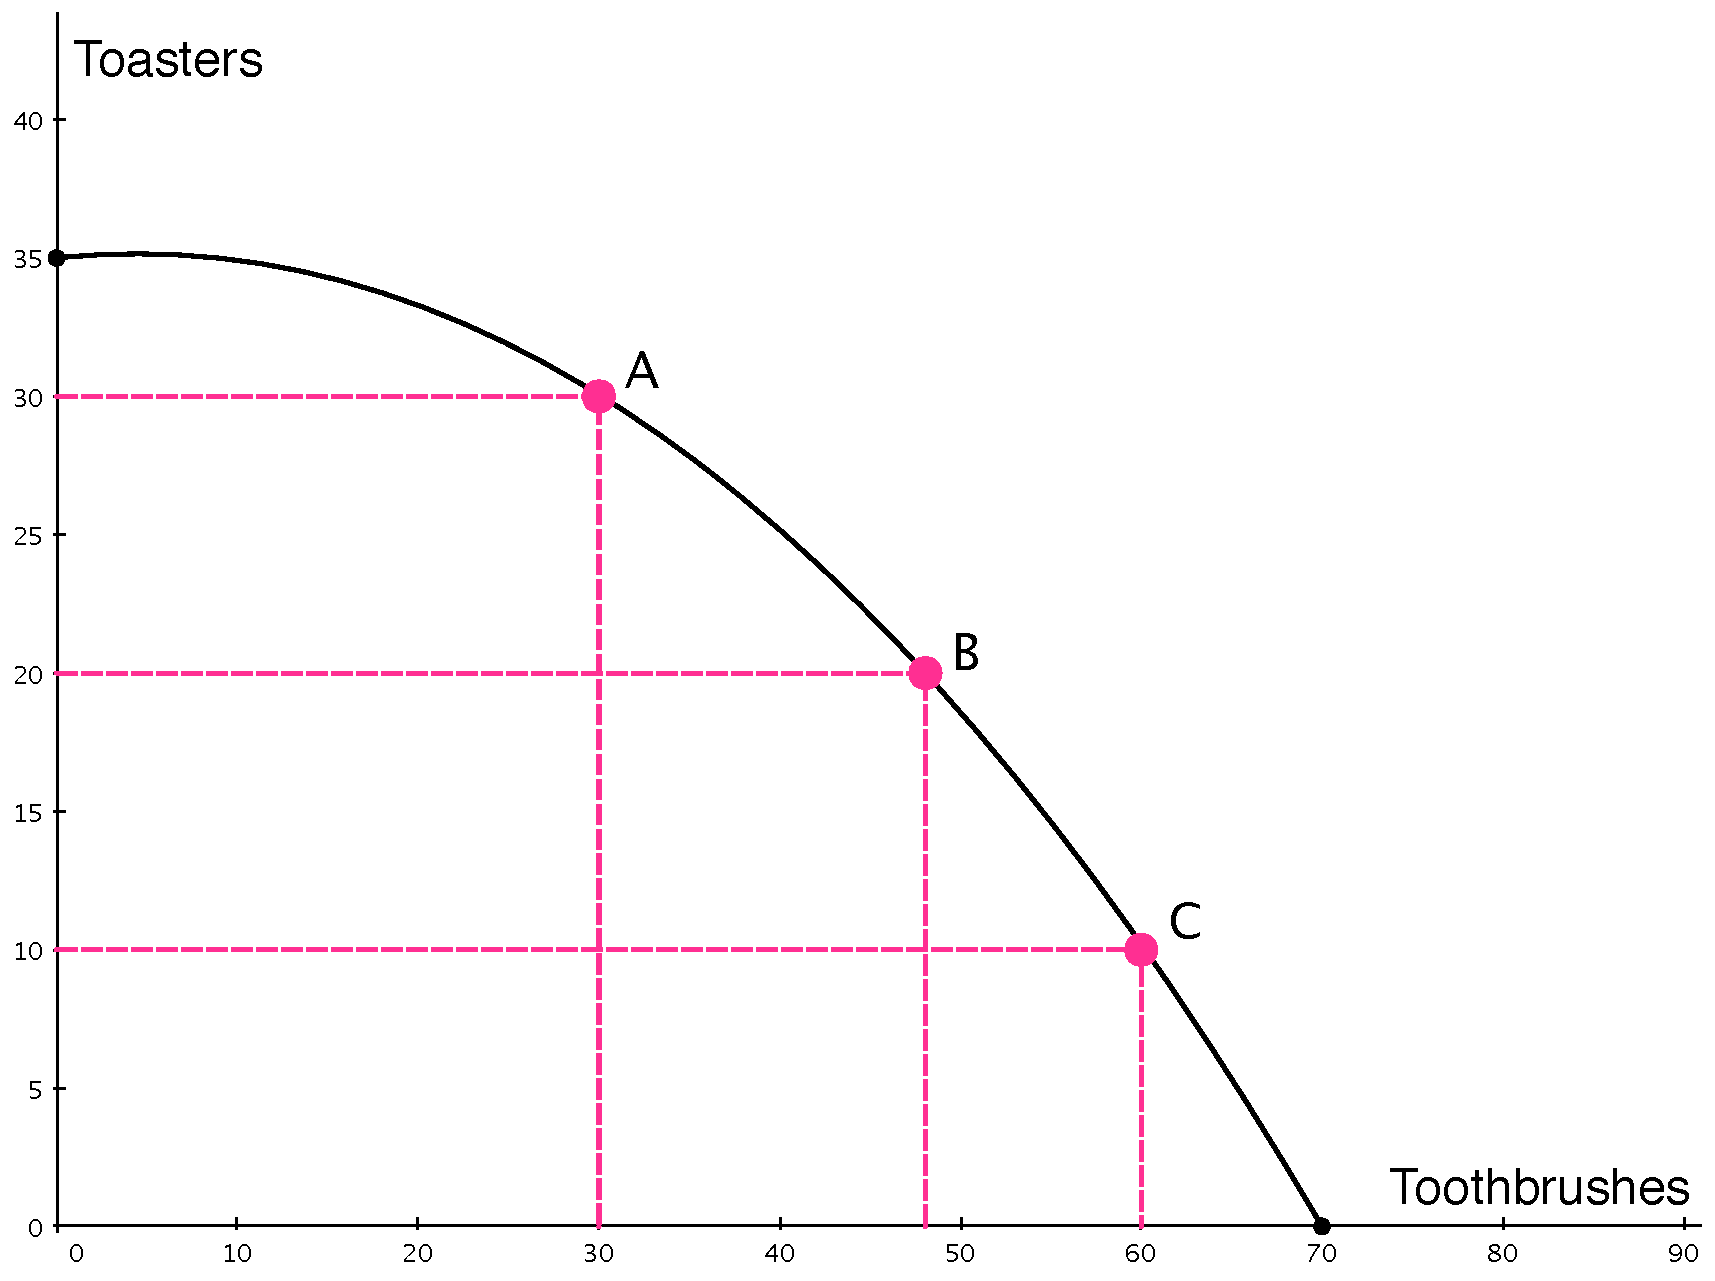
\includegraphics[scale=.3]{hw1_plot1.pdf}
	\caption{Production Possibilities Frontier}
	\label{fig1}
\end{figure}

Which of the following statements is TRUE?

\begin{choices}
	\choice The opportunity cost of toothbrushes is greater at point A than at point C.
	\CorrectChoice The opportunity cost of toasters is greater at point A than at point C.
	\choice The opportunity cost of toasters is greater at point C than at point A.
	\choice The opportunity cost of toothbrushes and toasters remains the same at all points.
\end{choices}

\question A new ad campaign, \textit{Hungry for Apples?}, uses various famous celebrities to promote the benefits and ``hipness'' of apples. Simultaneously, an influx of migrant workers drives the wage of apple farm laborers down. Given this, we can say that

\begin{choices}
	\choice the price of apples will decrease, while the change in the quantity bought and sold will be ambiguous.
	\CorrectChoice the quantity of apples bought and sold will increase, while the change in the price will be ambiguous.
	\choice the price of apples will increase, while the change in the quantity bought and sold will be ambiguous.
	\choice the quantity of apples bought and sold will decrease, while the change in the price will be ambiguous.
	\choice none of the above are true.
\end{choices}

\question Paul is a tutor for economics and he is debating whether or not to increase or decrease the price of his services. He has analyzed the market and found that the price elasticity of demand for economics tutors is 0.25 at his current price point. Given this, if Paul wants to increase his total revenue, he should \blank his price because \blank.

\begin{choices}
	\CorrectChoice increase; the price effect will be proportionately larger than the quantity effect
	\choice decrease; the price effect will be proportionately larger than the quantity effect
	\choice increase; the quantity effect will be proportionately larger than the price effect
	\choice decrease; the quantity effect will be proportionately larger than the price effect
\end{choices}





\question A subsidy provided in a market with no externalities will create a deadweight loss because 

\begin{choices}
	\choice it will reduce the number of transactions taking place, leading to unrealized gains from trade.
\CorrectChoice it will increase the number transactions taking place, leading to inefficient transactions.
	\choice it will decrease both consumer and producer surplus.
	\choice the increase in consumer and producer surplus is greater than the cost of the subsidy.
\end{choices}



\question In the market for low-skill labor, the equilibrium wage is \$5 an hour. There is currently a minimum wage of \$7.25 in place. If the government decides to increase the minimum wage to \$8 an hour, there will be a(n) \blank in unemployment, which will be largest if \blank.

\begin{choices}
	\choice decrease; labor supply and demand are elastic.
	\CorrectChoice increase; labor supply and demand are elastic.
	\choice increase; labor supply and demand are inelastic.
	\choice decrease; labor supply and demand are inelastic.
\end{choices}

\newpage

\question The imposition of a binding minimum wage in the market for labor will \blank surplus to workers and \blank total surplus in the market.
\begin{choices}
	\choice increase; increase
	\choice decrease; increase
	\choice decrease; decrease
	\CorrectChoice increase; decrease
\end{choices}



\question Which of the following statements accurately describes the relationship between the size of a per-unit tax and the size of the associated loss in total surplus?

\begin{choices}
	\choice As the size of the per-unit tax increases, the deadweight loss incurred decreases regardless of how high the tax is.
	\choice As the size of the per-unit tax increases, the deadweight loss incurred will increase initially, but will decrease after some point.
	\CorrectChoice As the size of the per-unit tax increases, the deadweight loss incurred increases regardless of how high the tax is.
	\choice As the size of the per-unit tax increases, the deadweight loss incurred will decrease initially, but will increase after some point.
\end{choices}

\question John is debating whether or not ride his bike to school today. His mom always yells at him because he spent \$800 to buy the bike two months ago, but he never seems to ride it. As a rational individual, John should

\begin{choices}
	\choice always ride his bike to school in order to ``get his money's worth'' on the \$800 he spent on it.
	\choice only ride his bike to school if the marginal benefit exceeds the \$800
	 cost of the bicycle.
	\CorrectChoice only ride his bike to school if the marginal benefit exceeds the marginal cost of riding the bicycle.
	\choice never ride his bike to school because his marginal benefit of riding will never exceed \$800.
\end{choices}

\question Suppose that a tropical storm in Florida destroys various orange growing orchards. As a result, if we were analyzing the market for oranges, we could (in theory)

\begin{choices}
	\CorrectChoice calculate the price elasticity of demand, but not the price elasticity of supply.
	\choice calculate the price elasticity of supply, but not the price elasticity of demand.
	\choice calculate the price elasticity of both supply and demand.
	\choice calculate the price elasticity of neither supply or demand.
\end{choices}

\question In the market for limes, total surplus is currently \$1,500. Which of the following would cause total surplus in the market to increase?

\begin{choices}
	\choice Either a decrease in demand, supply, or both.
	\CorrectChoice Either an increase in demand, supply, or both. 
	\choice An increase in demand only.
	\choice An increase in supply only.
	\choice None of the above.
\end{choices}

\newpage

\question How many of the following statements are \underline{normative}?

\begin{enumerate}[i.]
	\item ``An influx of migrants will decrease wages for native workers and lead to less native workers being employed.''
	\item ``We should increase the minimum wage because the loss in unemployment is outweighed by the gain in wage payments made to workers.''
	\item ``Increasing labor market opportunities for women in developing countries leads to increased labor force participation.''
	\item ``If migrant workers are complements to native workers, then an increase in migration will lead to an increase in wages to native workers in both the short and long-run.'' 
\end{enumerate}

\begin{choices}
	\choice 2
	\choice 4
	\choice 3
	\CorrectChoice 1
	\choice 0
\end{choices}

\question How many of the following statements \textit{could} cause the equilibrium price of drugs to decrease, but cause the equilibrium quantity to increase?

\begin{enumerate}[i.]
	\item A government program designed to crackdown on drug dealers is put into effect.
	\item The government expands a drug education program that educates individuals about the dangers of long-term drug use. 
	\item Both the 	``crackdown'' and drug education programs are put into effect simultaneously.
	\item The government legalizes drug use, leading to a surge of individuals ``experimenting'' with drug use. 
\end{enumerate}

\begin{choices}
	\choice 1
	\CorrectChoice 0
	\choice 2
	\choice 4
	\choice 3
\end{choices}



\question Which of the following statements is FALSE?

\begin{choices}
	\choice An individual must have an absolute advantage in producing a good if they can produce more of that good using the same number of inputs as other individuals.
	\choice An individual must have an absolute advantage in producing a good if they can produce the same amount of that good using fewer inputs as other individuals.
	\CorrectChoice An individual must have an absolute advantage in producing a good if they can produce more of that good using more inputs than other individuals.
	\choice An individual has the comparative advantage in producing a good if their opportunity cost of producing that good is lower than all other individuals.
	\choice All of the above are true.
\end{choices}


\question Suppose Kenya and Sri Lanka have the opportunity costs of producing limes and oranges outlined in  Table \ref{blah}. 

\begin{table}[H]
\caption{Opportunity cost of one:}
\centering
\begin{tabular}{ c|c|c} 
	
	& Lime & Orange \\
	\hline
	Kenya & 1/12 & $x$  \\
	Sri Lanka & $y$  & 8  \\
\end{tabular}
\label{blah}
\end{table}.

Given this information, we can say that

\begin{choices}
	\CorrectChoice Kenya has the comparative advantage in producing limes and Sri Lanka has the comparative advantage in producing oranges.
	\choice Kenya has the comparative advantage in producing oranges and Sri Lanka has the comparative advantage in producing limes.
	\choice Kenya has the absolute advantage in producing oranges and Sri Lanka has the absolute advantage in producing limes.
	\choice Kenya has the absolute advantage in producing limes and Sri Lanka has the absolute advantage in producing oranges.
	\choice there is not enough information to answer this question.
\end{choices}




\end{questions}

\end{document}